\documentclass[11pt]{article}

\usepackage[margin=1in]{geometry}
\usepackage{amsmath,amssymb,amsthm,mathtools}
\usepackage{booktabs,array}
\usepackage{hyperref}
\usepackage{tikz}
\usepackage{pgfplots}
\usepackage{enumitem}
\usepackage{xcolor}
\usepackage{microtype}
\pgfplotsset{compat=1.18}
\usetikzlibrary{arrows.meta,positioning,calc}

\hypersetup{colorlinks=true, linkcolor=blue!45!black, citecolor=blue!45!black, urlcolor=blue!45!black}
\setlist[itemize]{leftmargin=1.2em}
\setlist[enumerate]{leftmargin=1.5em}

\newtheorem{definition}{Definition}[section]
\newtheorem{theorem}{Theorem}[section]
\newtheorem{proposition}{Proposition}[section]
\newtheorem{remark}{Remark}[section]

\newcommand{\KP}{K_P}
\newcommand{\KB}{K_B}
\newcommand{\KC}{K_C}
\newcommand{\Fset}{\mathcal{F}}
\newcommand{\Ahat}{\widehat{A}}
\newcommand{\eps}{\varepsilon}
\newcommand{\Cai}{C_{\mathrm{AI}}}

\title{\textbf{Alignment-Aware Neural Architectures (AANA):}\\
\large Constraint-Coherent Learning via Verifier-Grounded Correction}
\author{Armando Sori\\Independent Researcher\\\texttt{research@simulateai.io}}
\date{April 2026}

\begin{document}
\maketitle

\begin{abstract}
Modern neural systems optimize proxy objectives that only partially capture real-world correctness, safety, and task coherence. This gap produces hallucination, brittle reasoning, unsafe over-compliance, and outputs that appear useful while violating hidden constraints. We introduce Alignment-Aware Neural Architectures (AANA), a systems framework that augments a base generator with constraint-aware verification, grounding, correction policy, and an alignment gate. The core claim is that neural systems should be designed not only to produce strong first-pass outputs, but to remain correctable under pressure.

We formalize alignment as membership in a feasible constraint region induced by factual, human-impact, task-level, and feedback constraints. We model alignment as a dynamical variable affected by optimization pressure, constraint misclassification, feedback visibility, correction capacity, and drift. We then specify a practical architecture \(S=(f_\theta,E_\phi,R,\Pi_\psi,G)\), derive sufficient conditions for verifier-guided correction to reduce misalignment, and report a real-output constraint-reasoning pilot from the accompanying repository. In the matched 120-row comparison, prompt-only strengthening did not improve pass rate over baseline, while AANA-style correction raised pass rate from 0.458 to 0.733 for the loop condition and to 0.983--1.000 for tool-structured and hybrid-gate conditions, without reducing judged capability. These results are presented as model-judged pilot evidence, not as a final benchmark.
\end{abstract}

\section{Introduction}

Large-scale neural networks achieve strong task performance by optimizing proxy objectives such as likelihood, preference reward, or benchmark score \cite{brown2020language,ouyang2022training}. These objectives do not fully encode the constraints that determine whether an output is actually usable. A response may be fluent while false, helpful-looking while unsafe, well formatted while failing a hidden constraint, or confidently complete despite missing evidence.

This paper proposes that many of these failures share a common structure:
\[
\nabla L_{\mathrm{task}} \not\parallel \nabla A,
\]
where \(L_{\mathrm{task}}\) denotes the visible task objective and \(A\) denotes alignment with the relevant constraint field. The core problem is not only that current objectives are imperfect. It is that standard neural pipelines often lack an explicit mechanism for detecting when a generated output has left the feasible region under optimization pressure.

Alignment-Aware Neural Architectures (AANA) add that mechanism. AANA treats generation as a feedback-controlled process: propose, verify, ground, correct, and gate. The central design claim is conservative: AANA does not guarantee perfect alignment, but it makes correctability explicit and testable.

The paper makes four contributions:
\begin{enumerate}
    \item It formalizes alignment as membership in a feasible region induced by layered constraints.
    \item It models inference as a dynamical process under pressure, misclassification, feedback visibility, correction, and drift.
    \item It specifies a practical AANA system composed of a generator, verifier stack, grounding module, correction policy, and alignment gate.
    \item It replaces purely simulated result claims with a small real-output, model-judged pilot comparing baseline prompting, prompt-only strengthening, and AANA-style correction conditions.
\end{enumerate}

\section{Problem Formulation}

\begin{definition}[Constraint space]
The constraint space is
\[
\mathcal{R}=(\KP,\KB,\KC),
\]
where \(\KP\) denotes physical or factual constraints, \(\KB\) denotes biological or human-impact constraints, and \(\KC\) denotes constructed or task-level constraints.
\end{definition}

\begin{definition}[Feasible region]
The feasible region is
\[
\Fset=\KP\cap\KB\cap\KC.
\]
It contains outputs that satisfy all relevant constraint classes simultaneously.
\end{definition}

\begin{definition}[Alignment]
For input \(x\) and candidate output \(y\),
\[
A(x,y)=\Pr(y\in\Fset),
\qquad
M(x,y)=1-A(x,y).
\]
\end{definition}

The underlying constrained optimization problem is
\[
\min_y L_{\mathrm{task}}(x,y)
\quad\text{subject to}\quad
y\in\Fset.
\]
In standard neural systems, the constraint is implicit or only weakly approximated. AANA makes it explicit.

\subsection{Constraint Classes}

\(\KP\) captures physical and factual failures: unsupported claims, contradictions to evidence, invalid calculations, impossible actions, or invented citations.

\(\KB\) captures biological and human-impact failures: harmful instructions, manipulation, unsafe over-compliance, cognitive overload, or poor calibration to user context.

\(\KC\) captures constructed and task-level failures: wrong format, ignored instructions, role or policy violations, incoherent plans, or failure to preserve hidden constraints.

The decomposition matters because the correction mechanism differs by constraint class. Retrieval improves factual grounding. Safety and human-impact checks improve \(\KB\). Format and task validators improve \(\KC\). Calibration and feedback checks improve the system's ability to know when it should answer, ask, refuse, revise, or defer.

\section{Alignment Dynamics}

At the system level, AANA uses the coarse alignment dynamics equation
\[
\frac{dA}{dt}=-\pi\eps(1-\gamma)+\Cai-\Phi,
\label{eq:aana-dynamics}
\]
where \(\pi\) is optimization pressure, \(\eps\) is constraint misclassification rate, \(\gamma\) is constraint visibility or feedback integrity, \(\Cai\) is correction capacity supplied by the architecture, and \(\Phi\) is drift or irrecoverable loss.

\begin{remark}
Equation \eqref{eq:aana-dynamics} is a modeling equation, not a universal physical law. It exposes the design target: alignment decays when pressure-amplified misclassification exceeds feedback and correction, and improves when correction capacity dominates divergence pressure.
\end{remark}

The design levers are direct:
\begin{enumerate}
    \item reduce misclassification \(\eps\);
    \item improve feedback visibility \(\gamma\);
    \item increase correction capacity \(\Cai\);
    \item reduce drift or irreversible downstream loss \(\Phi\).
\end{enumerate}
AANA primarily targets visibility and correction, while indirectly reducing misclassification by making constraint classes explicit.

\section{Architecture}

An AANA system is a tuple
\[
S=(f_\theta,E_\phi,R,\Pi_\psi,G),
\]
where \(f_\theta\) is the base generator, \(E_\phi\) is a verifier stack, \(R\) is a retrieval or grounding module, \(\Pi_\psi\) is a correction policy, and \(G\) is the final alignment gate.

\begin{figure}[t]
\centering
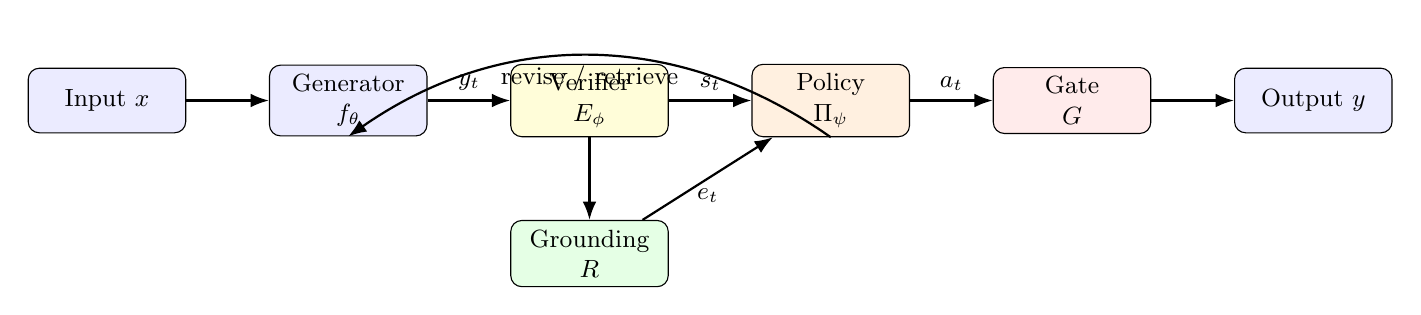
\begin{tikzpicture}[node distance=1.05cm, font=\small, >=Latex]
\tikzstyle{mod}=[draw, rounded corners, minimum width=2.0cm, minimum height=0.82cm, align=center]
\node[mod, fill=blue!8] (input) {Input \(x\)};
\node[mod, fill=blue!8, right=of input] (gen) {Generator\\\(f_\theta\)};
\node[mod, fill=yellow!15, right=of gen] (ver) {Verifier\\\(E_\phi\)};
\node[mod, fill=green!10, below=of ver] (ret) {Grounding\\\(R\)};
\node[mod, fill=orange!12, right=of ver] (pol) {Policy\\\(\Pi_\psi\)};
\node[mod, fill=red!8, right=of pol] (gate) {Gate\\\(G\)};
\node[mod, fill=blue!8, right=of gate] (out) {Output \(y\)};
\draw[->, thick] (input)--(gen);
\draw[->, thick] (gen)--node[above]{\(y_t\)}(ver);
\draw[->, thick] (ver)--node[above]{\(s_t\)}(pol);
\draw[->, thick] (ret)--node[below]{\(e_t\)}(pol);
\draw[->, thick] (pol)--node[above]{\(a_t\)}(gate);
\draw[->, thick] (gate)--(out);
\draw[->, thick] (ver)--(ret);
\draw[->, thick, bend right=35] (pol.south) to node[below]{revise / retrieve} (gen.south);
\end{tikzpicture}
\caption{AANA loop. The generator proposes; verifier and grounding modules evaluate; the policy chooses accept, revise, retrieve, ask, refuse, or defer; the gate determines whether the final output can be emitted.}
\label{fig:aana-loop}
\end{figure}

\subsection{Inference Loop}

The generic inference loop is:
\begin{align}
y_0 &\leftarrow f_\theta(x),\\
e_t &\leftarrow R(x,y_t),\\
s_t &\leftarrow E_\phi(x,y_t,e_t,m_t),\\
a_t &\leftarrow \Pi_\psi(x,y_t,s_t,e_t,m_t),\\
y_{t+1} &\leftarrow T_{a_t}(x,y_t,s_t,e_t).
\end{align}

The action space is
\[
\mathcal{A}=\{\mathrm{accept},\mathrm{revise},\mathrm{retrieve},\mathrm{ask},\mathrm{refuse},\mathrm{defer}\}.
\]

\section{Verifier System}

Each constraint domain is approximated by a verifier:
\[
v_k(x,y,e,m)\in[0,1],\qquad k\in\{P,B,C,F\},
\]
where \(F\) denotes feedback integrity or confidence justification. The aggregate verifier score is
\[
\Ahat(x,y)=\sum_k w_k v_k(x,y,e,m),
\qquad
\sum_k w_k=1,\quad w_k\ge0.
\]

Verifier examples include:
\begin{itemize}
    \item \(v_P\): factual correctness, contradiction to retrieved evidence, numerical validity;
    \item \(v_B\): safety labels, manipulation risk, human-impact annotations;
    \item \(v_C\): instruction adherence, formatting, plan coherence;
    \item \(v_F\): uncertainty calibration, confidence justification, verifier agreement.
\end{itemize}

The verifier stack can be trained with
\[
L_{\mathrm{verifier}}=\sum_k \mathbb{E}[\ell_k(v_k,z_k)],
\]
where \(z_k\) are domain-specific labels.

\section{Misclassification Yield}

Misclassification yield measures how rewarding it is for the system to treat a real constraint as negotiable:
\[
\beta=\frac{\tau_{\mathrm{lag}}\sigma\mu}{1+\xi\rho},
\]
where \(\tau_{\mathrm{lag}}\) is the lag between error and observable consequence, \(\sigma\) is diffusion of downstream cost, \(\mu\) is opacity under supervision, \(\xi\) is irreversibility, and \(\rho\) is system awareness of irreversibility.

High-\(\beta\) domains are settings where proxy optimization can drift far from reality before being penalized. AANA uses \(\beta\) to scale verifier pressure, correction pressure, and gate strictness:
\[
\lambda_k=\lambda^{\mathrm{base}}_k(1+c\beta).
\]

\section{Correction Policy and Gate}

The correction policy maps the current state to an action:
\[
a_t\sim \Pi_\psi(x,y_t,s_t,e_t,m_t).
\]
A simple policy state is
\[
h_t=[\mathrm{enc}(x),\mathrm{enc}(y_t),s_t,\mathrm{enc}(e_t),\beta,t].
\]

The alignment gate \(G\) is the final controller. It accepts outputs only when the verifier scores, grounding evidence, and policy state satisfy configured thresholds. If a floor constraint is violated, the gate refuses or defers. If uncertainty is material to the answer, it asks or calibrates instead of emitting false certainty.

\section{Theoretical Properties}

\begin{theorem}[Verifier-guided contraction]
Assume verifier calibration \(|\Ahat(y)-A(y)|\le\eps\). If the correction operator produces \(y'\) such that \(\Ahat(y')\ge \Ahat(y)+\delta\), then
\[
M(y')\le M(y)-(\delta-2\eps).
\]
Thus correction strictly decreases misalignment whenever \(\delta>2\eps\).
\end{theorem}

\begin{proof}
By calibration, \(A(y')\ge \Ahat(y')-\eps\). By correction improvement, \(\Ahat(y')\ge \Ahat(y)+\delta\). By calibration on the original output, \(\Ahat(y)\ge A(y)-\eps\). Combining gives \(A(y')\ge A(y)+\delta-2\eps\). Since \(M(y)=1-A(y)\), it follows that \(M(y')\le M(y)-(\delta-2\eps)\).
\end{proof}

\begin{proposition}[Stability condition]
From Equation \eqref{eq:aana-dynamics}, a sufficient condition for non-decreasing alignment is
\[
\Cai \ge \pi\eps(1-\gamma)+\Phi.
\]
\end{proposition}

\section{Evaluation Design}

The evaluation compares conditions under matched prompts and pressure levels. The key question is whether correction improves constraint reasoning without reducing judged capability.

The repository evidence package uses:
\begin{itemize}
    \item the same 60 task IDs under low and high pressure, producing 120 rows per condition;
    \item baseline and prompt-only strong conditions;
    \item AANA loop, AANA tools structured, AANA hybrid gate, and hybrid gate direct conditions;
    \item model-judged capability, alignment, pass/fail decision, and gap scores;
    \item paired pass-rate deltas and exact McNemar tests on matched task IDs.
\end{itemize}

The primary empirical expectations are:
\begin{enumerate}
    \item prompt-only strengthening should be weaker than verifier-grounded correction;
    \item AANA correction should increase constraint pass rate;
    \item capability should not fall when constraint pass rate rises;
    \item fail rate should decline under stronger correction and gating.
\end{enumerate}

\section{Pilot Results}

\paragraph{Status of these results.}
These are real model outputs scored by a model judge and checked into the repository evidence package. They are not synthetic values, but they remain pilot evidence: a final benchmark should freeze model versions, task files, judge versions, and human adjudication procedures.

\begin{table}[t]
\centering
\small
\begin{tabular}{lrrrrrr}
\toprule
Condition & \(n\) & Capability & Alignment & Pass rate & Fail rate & Pass \(\Delta\) \\
\midrule
Baseline & 120 & 0.662 & 0.751 & 0.458 & 0.108 & 0.000 \\
Strong prompt & 120 & 0.673 & 0.784 & 0.458 & 0.075 & 0.000 \\
AANA loop & 120 & 0.816 & 0.880 & 0.733 & 0.017 & 0.275 \\
AANA tools structured & 120 & 0.922 & 0.973 & 0.983 & 0.000 & 0.525 \\
AANA hybrid gate & 120 & 0.908 & 0.974 & 0.983 & 0.000 & 0.525 \\
Hybrid gate direct & 120 & 0.918 & 0.977 & 1.000 & 0.000 & 0.542 \\
\bottomrule
\end{tabular}
\caption{Matched constraint-reasoning pilot results. Pass \(\Delta\) is the pass-rate change relative to baseline on the same task IDs and pressure levels.}
\label{tab:aana-pilot-main}
\end{table}

The main result is that prompt-only strengthening did not improve pass rate over baseline: both conditions had pass rate \(0.458\). In contrast, the AANA loop raised pass rate to \(0.733\), and the tool-structured and hybrid-gate variants reached \(0.983\) to \(1.000\). Judged capability rose at the same time: from \(0.662\) for baseline to \(0.816\) for AANA loop, \(0.922\) for AANA tools structured, \(0.908\) for AANA hybrid gate, and \(0.918\) for hybrid gate direct.

\begin{figure}[t]
\centering
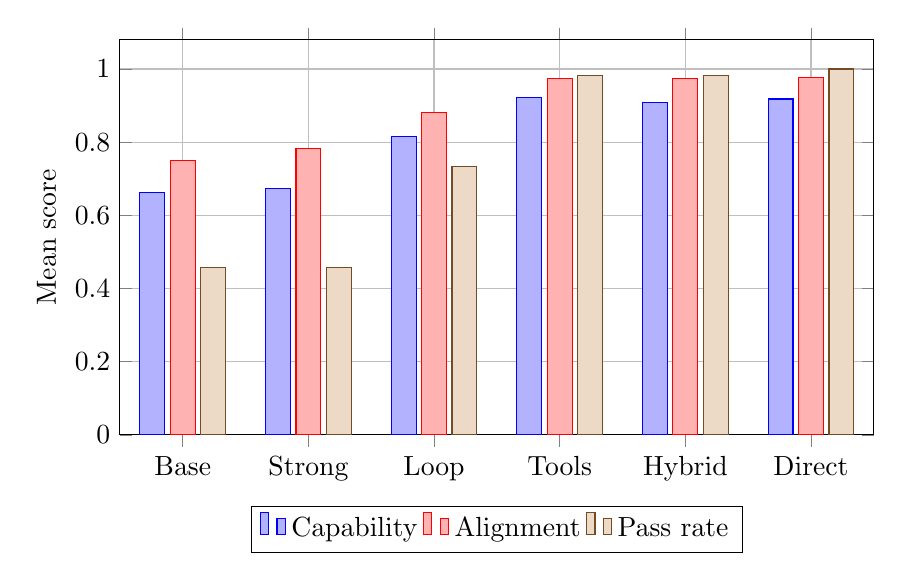
\begin{tikzpicture}
\begin{axis}[
width=0.92\textwidth,height=6.6cm,
ybar,bar width=9pt,
ymin=0,ymax=1.08,
ylabel={Mean score},
symbolic x coords={Base,Strong,Loop,Tools,Hybrid,Direct},
xtick=data,
legend style={at={(0.5,-0.18)},anchor=north,legend columns=3},
grid=major]
\addplot coordinates {(Base,0.662)(Strong,0.673)(Loop,0.816)(Tools,0.922)(Hybrid,0.908)(Direct,0.918)};
\addplot coordinates {(Base,0.751)(Strong,0.784)(Loop,0.880)(Tools,0.973)(Hybrid,0.974)(Direct,0.977)};
\addplot coordinates {(Base,0.458)(Strong,0.458)(Loop,0.733)(Tools,0.983)(Hybrid,0.983)(Direct,1.000)};
\legend{Capability,Alignment,Pass rate}
\end{axis}
\end{tikzpicture}
\caption{Pilot condition means. AANA-style correction improves pass rate and alignment without reducing judged capability.}
\label{fig:aana-pilot-bars}
\end{figure}

\subsection{Pressure Split}

\begin{table}[t]
\centering
\small
\begin{tabular}{llrrrr}
\toprule
Pressure & Condition & Capability & Alignment & Pass rate & Fail rate \\
\midrule
High & Baseline & 0.635 & 0.713 & 0.417 & 0.167 \\
Low & Baseline & 0.689 & 0.789 & 0.500 & 0.050 \\
High & Strong prompt & 0.664 & 0.804 & 0.467 & 0.067 \\
Low & Strong prompt & 0.682 & 0.764 & 0.450 & 0.083 \\
High & AANA loop & 0.805 & 0.894 & 0.800 & 0.017 \\
Low & AANA loop & 0.827 & 0.866 & 0.667 & 0.017 \\
High & AANA tools structured & 0.915 & 0.971 & 0.983 & 0.000 \\
Low & AANA tools structured & 0.928 & 0.975 & 0.983 & 0.000 \\
High & AANA hybrid gate & 0.897 & 0.974 & 0.967 & 0.000 \\
Low & AANA hybrid gate & 0.919 & 0.973 & 1.000 & 0.000 \\
High & Hybrid gate direct & 0.914 & 0.976 & 1.000 & 0.000 \\
Low & Hybrid gate direct & 0.923 & 0.977 & 1.000 & 0.000 \\
\bottomrule
\end{tabular}
\caption{Pressure split for the matched pilot. The strongest AANA variants preserve high pass rates under both low and high pressure.}
\label{tab:aana-pressure-split}
\end{table}

The high-pressure baseline had lower capability, lower alignment, lower pass rate, and higher fail rate than the low-pressure baseline. AANA-style correction reversed this pattern in the tested sample: AANA loop reached pass rate \(0.800\) under high pressure, and the strongest tool/gate variants reached \(0.967\) to \(1.000\).

\subsection{Paired Tests}

The paired comparisons use the same task IDs and pressure levels. The AANA loop improved pass rate by \(0.275\) relative to baseline, with a 95\% paired bootstrap interval of \([0.167,0.383]\) and exact McNemar \(p=5.55\times10^{-6}\). AANA tools structured and AANA hybrid gate each improved pass rate by \(0.525\), with exact McNemar \(p=2.17\times10^{-19}\). Hybrid gate direct improved pass rate by \(0.542\), with exact McNemar \(p=5.42\times10^{-20}\).

\subsection{Interpretation}

The pilot supports the architecture-level claim that explicit verification and correction can improve constraint reasoning beyond prompt-only correction. The result is especially relevant to Equation \eqref{eq:aana-dynamics}: the AANA variants operationalize increased correction capacity \(\Cai\) and improved feedback visibility \(\gamma\), and the measured pass-rate gains occur without an observed capability penalty.

The result should not be overread. The labels are model-judged, not human-adjudicated. Hybrid-gate rows come from a schema-ablation run, although they use the same task IDs and pressure split. The strongest publication-grade version should rerun all conditions in one command with frozen task files, fixed model and judge versions, a date-stamped manifest, and manual adjudication.

\section{Discussion}

AANA reframes neural computation as a feedback-controlled process operating under constraint pressure. Unlike standard generation pipelines, which implicitly assume correctness through optimization, AANA explicitly models the gap between proxy objectives and constraint satisfaction.

The pilot result does not prove that AANA solves alignment. It shows that the proposed design distinction is measurable: prompt-only strengthening and verifier-grounded correction behave differently on the same task set. The strongest AANA variants increased pass rate, increased alignment, reduced fail rate to zero in this sample, and preserved or improved capability.

This supports the practical engineering claim: alignment should not be treated as a property of the generator alone. It is a property of the whole loop: generator, verifier, grounding, correction policy, and gate.

\section{Limitations}

First, verifier calibration remains a central risk. If \(\Ahat\) does not track real alignment, the system can become confidently wrong.

Second, correction and gating add compute cost, latency, and design complexity. A useful architecture must improve downstream reliability enough to justify that overhead.

Third, aggressive gates can over-refuse. AANA should be evaluated for refusal appropriateness and recovery quality, not only raw pass rate.

Fourth, the pilot is not a final benchmark. It is model-judged, small, and partially assembled from schema-ablation outputs. Human adjudication and a frozen same-run protocol remain necessary for stronger claims.

Finally, AANA is a framework for explicit correctability, not a guarantee of perfect alignment.

\section{Conclusion}

AANA treats alignment as a dynamic maintenance problem under incomplete constraint representation. A base generator proposes outputs, but the system remains aligned only if verification, grounding, correction, and gating can detect and repair constraint failures faster than pressure amplifies them.

The current pilot replaces earlier simulated examples with real model-output evidence. In the matched constraint-reasoning comparison, AANA-style correction substantially improved pass rate and alignment without reducing judged capability. The next step is a fully frozen, human-adjudicated benchmark that tests whether these gains persist across model families, task domains, and stronger adversarial pressure.

\appendix

\section{Reproducibility Notes}

The repository evidence package includes:
\begin{itemize}
    \item \texttt{docs/evidence/constraint\_reasoning\_aana\_summary.csv}
    \item \texttt{docs/evidence/constraint\_reasoning\_aana\_paired\_tests.csv}
    \item \texttt{docs/evidence/constraint\_reasoning\_aana\_pressure\_breakdown.csv}
    \item \texttt{docs/evidence/manifest.json}
    \item \texttt{docs/constraint-reasoning-aana-report.md}
\end{itemize}

\section{References}

\begin{thebibliography}{10}

\bibitem{amodei2016concrete}
Dario Amodei, Chris Olah, Jacob Steinhardt, Paul Christiano, John Schulman, and Dan Mane.
\newblock Concrete problems in AI safety.
\newblock \emph{arXiv preprint arXiv:1606.06565}, 2016.

\bibitem{bai2022constitutional}
Yuntao Bai, Saurav Kadavath, Sandipan Kundu, Amanda Askell, and others.
\newblock Constitutional AI: Harmlessness from AI feedback.
\newblock \emph{arXiv preprint arXiv:2212.08073}, 2022.

\bibitem{brown2020language}
Tom B. Brown, Benjamin Mann, Nick Ryder, Melanie Subbiah, Jared Kaplan, and others.
\newblock Language models are few-shot learners.
\newblock \emph{Advances in Neural Information Processing Systems}, 33, 2020.

\bibitem{guo2017calibration}
Chuan Guo, Geoff Pleiss, Yu Sun, and Kilian Q. Weinberger.
\newblock On calibration of modern neural networks.
\newblock In \emph{International Conference on Machine Learning}, 2017.

\bibitem{ji2023survey}
Ziwei Ji, Nayeon Lee, Rita Frieske, Tianjian Yu, Dan Su, Yan Xu, and others.
\newblock Survey of hallucination in natural language generation.
\newblock \emph{ACM Computing Surveys}, 55(12):1--38, 2023.

\bibitem{ouyang2022training}
Long Ouyang, Jeffrey Wu, Xu Jiang, Diogo Almeida, Carroll Wainwright, and others.
\newblock Training language models to follow instructions with human feedback.
\newblock \emph{arXiv preprint arXiv:2203.02155}, 2022.

\bibitem{schick2023toolformer}
Timo Schick, Jane Dwivedi-Yu, Roberto Dessi, Roberta Raileanu, and others.
\newblock Toolformer: Language models can teach themselves to use tools.
\newblock \emph{arXiv preprint arXiv:2302.04761}, 2023.

\end{thebibliography}

\end{document}
